\documentclass{article}
\usepackage{graphicx}
\title{Programming Assignment 1: Algorithm Implementation Project}
\author{Patrick Rumble}

\begin{document}
\maketitle

\section{What I built}
A simple GUI program using Aho-Corasick to match multiple patterns in a file, displaying the matches in a separate window. The program uses imgui, and takes an input file and patterns to filter.
\section{The Track-Specific Writeup}
The program has two main windows, and one optional window for benchmarking purposes. 
The user can input any number of patterns, an input file, and press the run button, and the results will show in the result window.
The benchmark window (enabled at compile time) allows for simulation of any number of patterns used to find matches in a simulated dataset, and compares the speed with that of std::string:;find.
\\

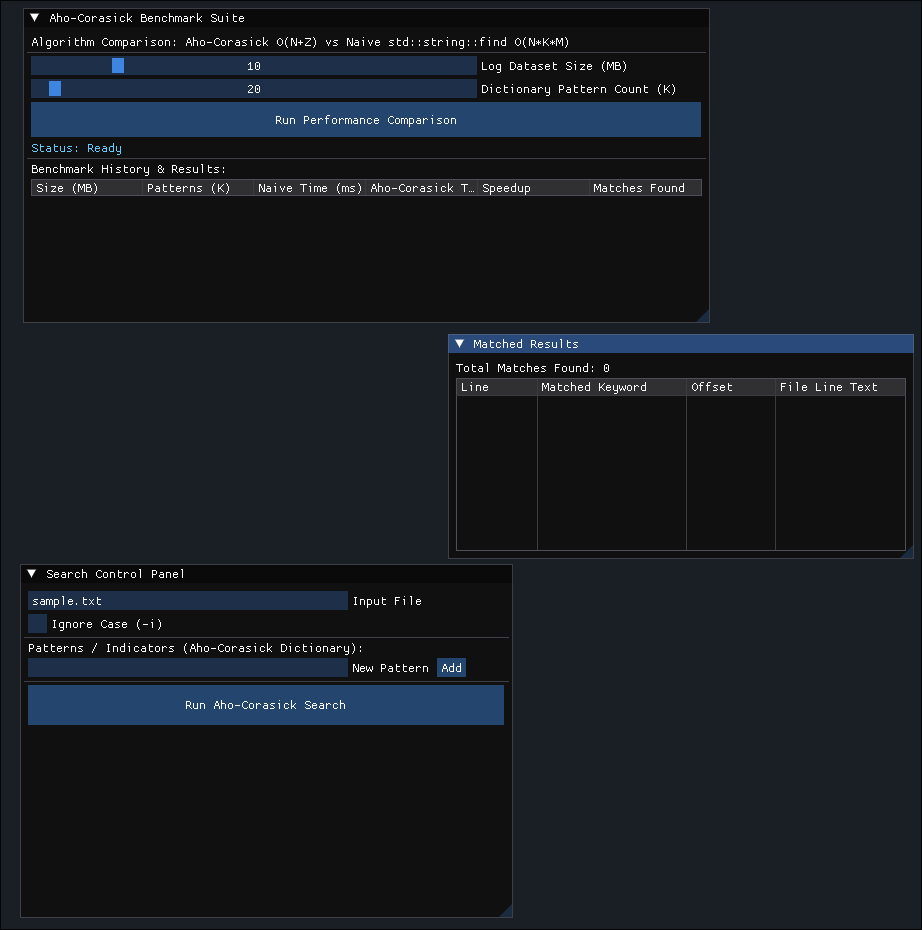
\includegraphics[width=1\textwidth]{program.png}
\pagebreak
\\
As is visible in the attached image, std::string::find easily wins on time at low pattern counts, but as the number of patterns increases, the Aho-Corasick time stays consistent, eventually winning.
\\\\
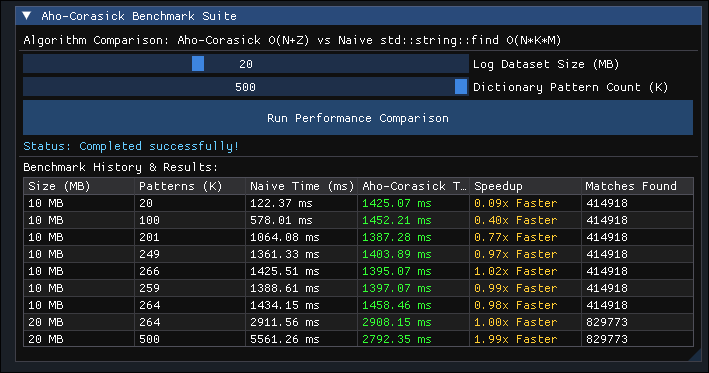
\includegraphics[width=1\textwidth]{benchmark_results.png}
The algorithm implementation sits inside the file ahocorasick.cpp. Code in this file is executed when the user clicks run, through the run\_async\_search function.
\section{What I learned}
Before working on this task I had not heard of Aho-Corasick, so everything about it was a learning experience. I was also highly suprised by how many patterns the Aho-Corasick implementation took to beat the std::string::find comparison.
\section{AI Use}
\subsection{Which Tools I Used}
For this task I primarily made use of Gemini's free tier, as this is one of the few AI tools I have used in the past.
\subsection{What I Used Them For}
Gemini was used to assist in writing the implementation, as well as provide feedback on ideas.
\subsection{Examples of Where AI Was Unhelpful}
Gemini produced some code with errors, for example when implementing the GUI, using ImVec2 instead of ImVec4 in its generated code, and leaving out arguments in glClear(). Additionally, when attempting to add further functionality to the GUI, it just generated a non-functional textbox.
\subsection{What I Understood and What I Took On Trust}
I have placed a lot of trust in Gemini when it comes to this task. I have no experience with GUI programs or CMake, and was heavily reliant on Gemini for the code involved.

\section{Video Walkthrough}
https://youtu.be/Nwdvl02RuFU
\end{document}